\Testart{Skript}
\Klasse{09}
\Fach{Informatik}
\Titel{Objektorientierte Programmierung mit Java}

\renewcommand{\Content}{
    
    \mysession{Stunde 1+2}{
        \Hefteintrag{1.7}{Programmieren: Sprachen}{
Beim Programmieren schreibt man präzise und unmissverständliche Befehle, die dann vom \LoesungLuecke{Compiler}{6cm}~in Maschinensprache übersetzt werden. 

Hierfür gibt es verschiedene Programmiersprachen mit jeweils einer festgelegte \emphColA{Grammatik und Rechtschreibung (=\LoesungLuecke{Syntax}{4cm})}. Dem gegenüber steht die \emphColC{Logik eines Programms (=~\LoesungLuecke{Semantik}{4cm})}, die weitgehend unabhängig von der Programmiersprache ist.

\vspace{0.2cm}
Bei den einsteigerfreundlichen \emphColA{block-basierten Sprachen wie Blockly oder Online-Karol} übernehmen die Blöcke und ihre Verbindungsmöglichkeiten weitgehend die Einhaltung des Syntax. Bei \emphColC{text-basierten Sprachen wie \LoesungLuecke{Java}{6cm}~oder \LoesungLuecke{Python}{6cm}} müssen die Entwickler:innen selbst auf deren Einhaltung achten. Diese Sprachen bieten dadurch aber auch weitaus mehr Möglichkeiten (\emph{man sagt auch: sie sind mächtiger}). 

Dieses Skript arbeitet parallel mit den blockbasierten Sprachen Blockly und Online-Karol und der weit verbreiteten text-basierten und \emphColA{objektorientierten} Sprache \emphColA{Java}.

}

        \begin{center}
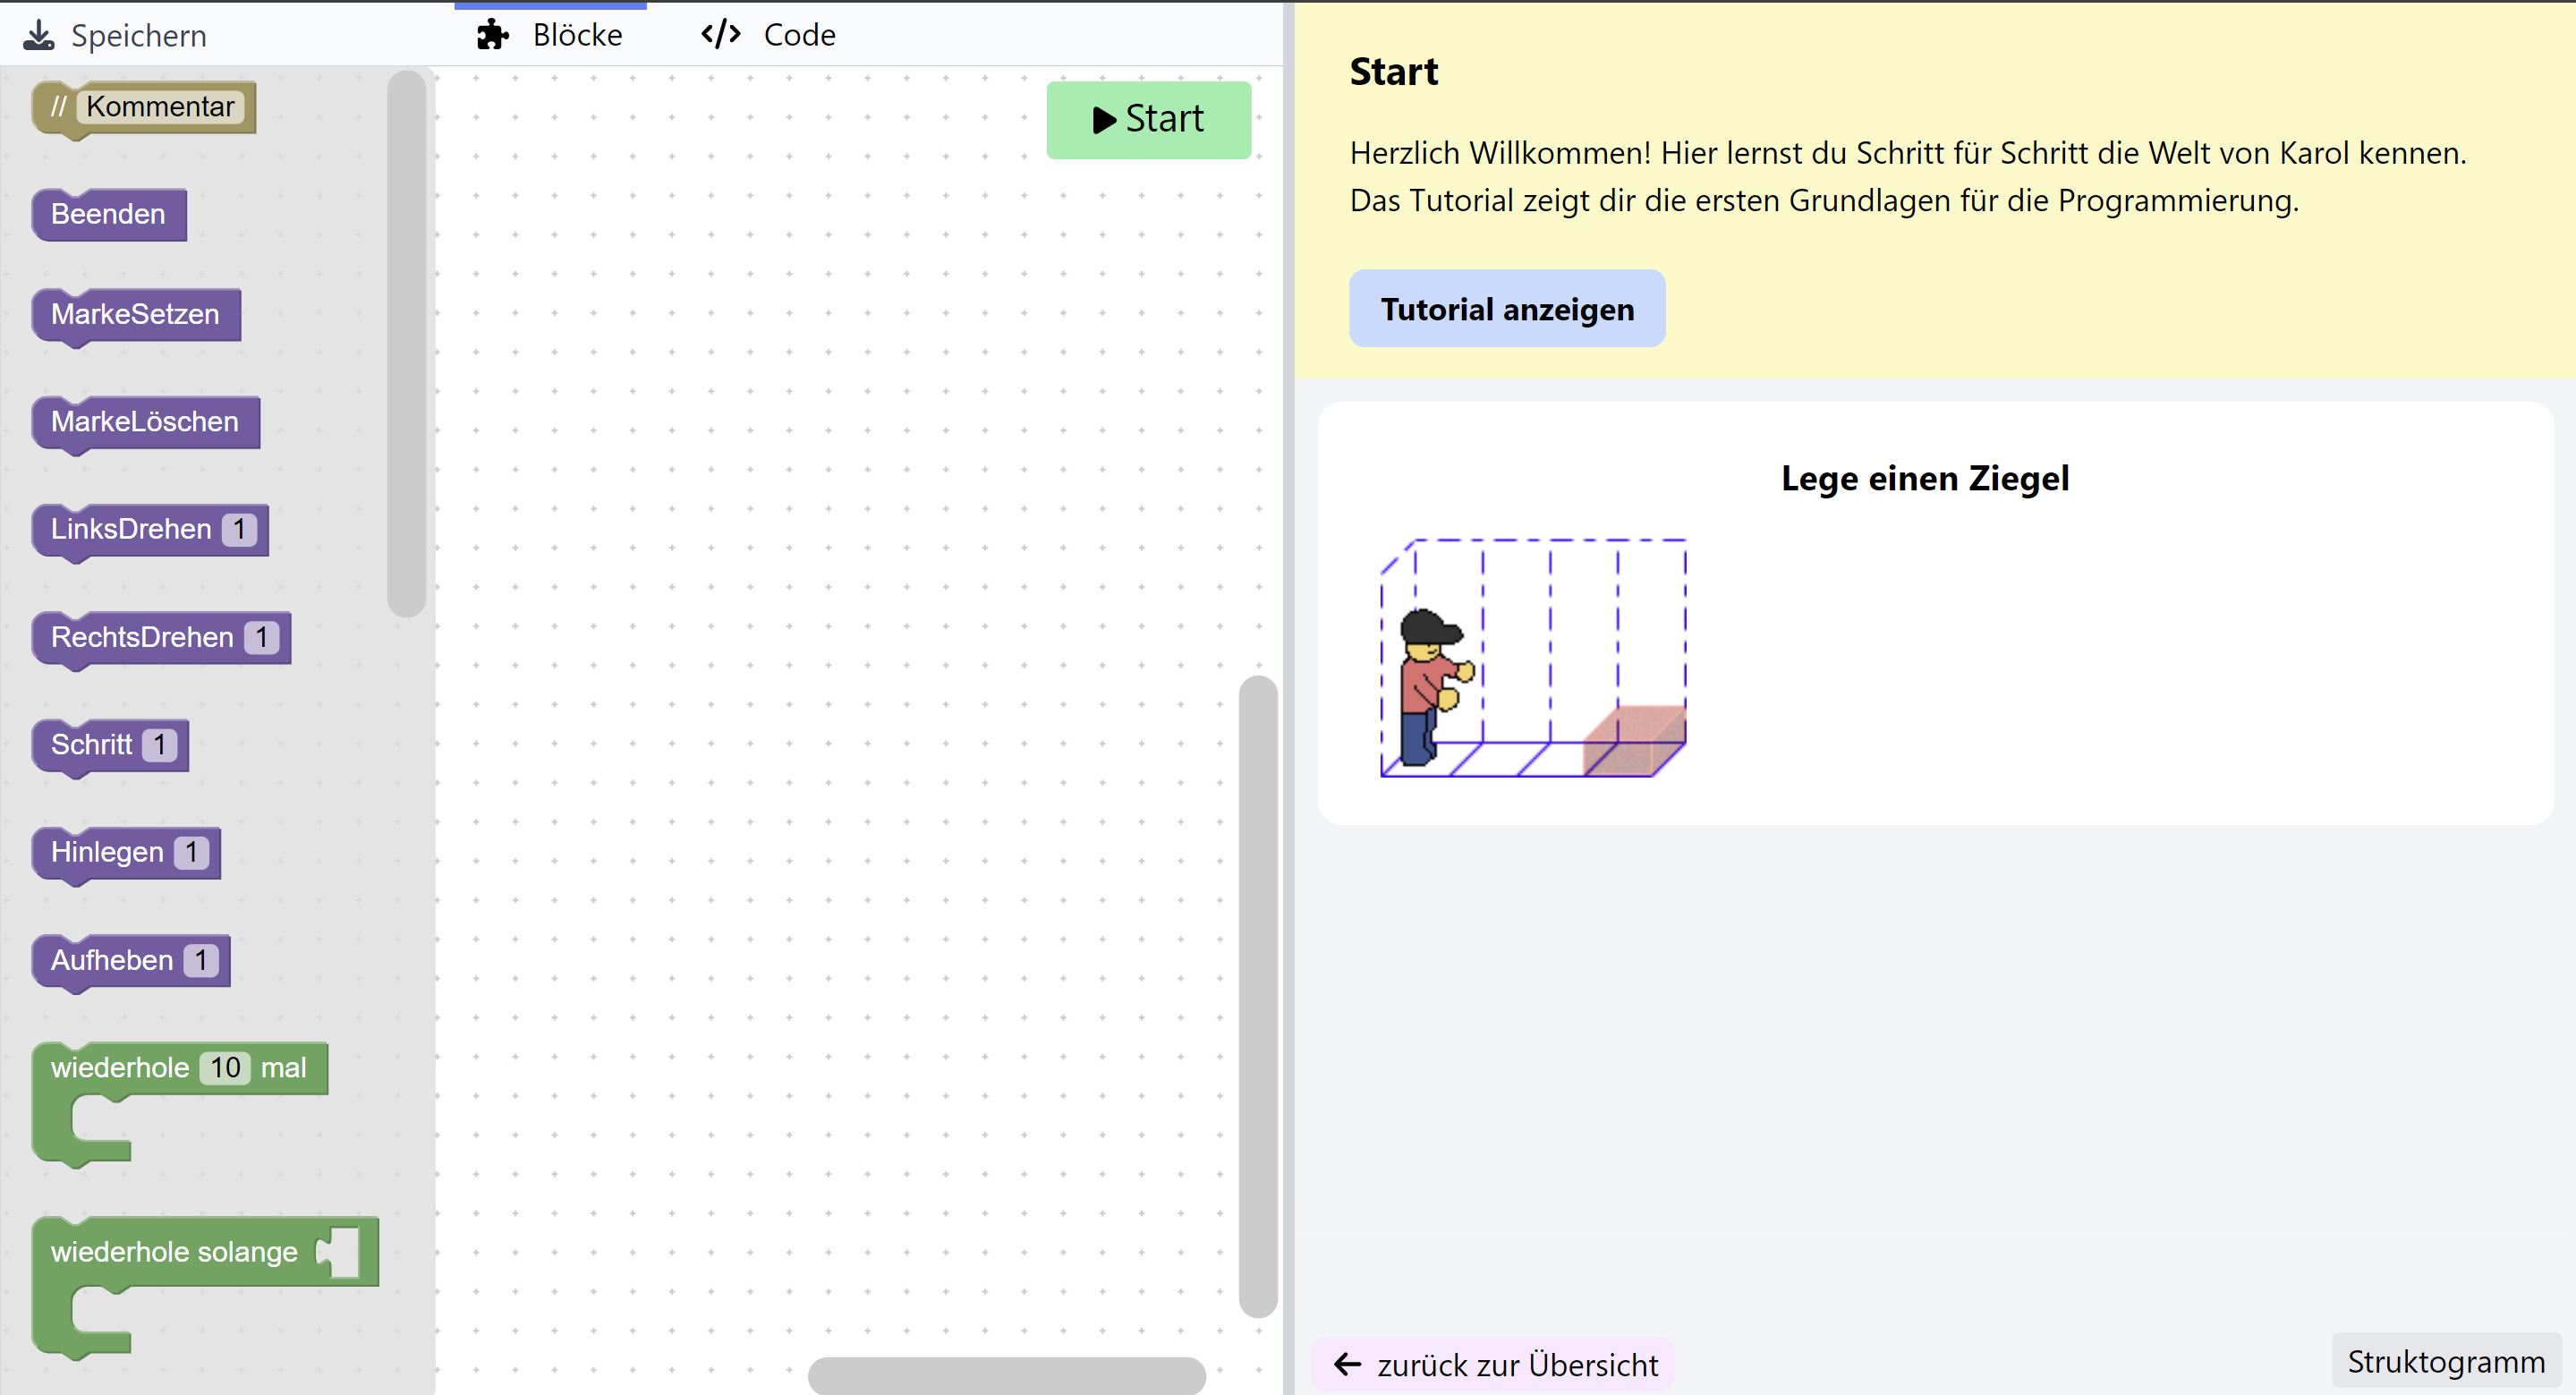
\includegraphics[width=0.85\textwidth]{_Aufgaben/BlocksAndJava/img/overview.png}
\end{center}

\Aufgabe{Karol-Java Übersetzung}{

\begin{enumerate}
    \item Bearbeite die Aufgaben von Robot Karol online: \url{karol.arrrg.de}
    \item Schalte in der Code-Ansicht die Sprache auf Java um und notiere auf dem AB jeweils zu welchem Java-Code der Block übersetzt wird. Achte hierbei auf Einrückungen!
\end{enumerate}


\begin{tabularx}{\textwidth}{p{4cm}X}

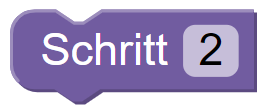
\includegraphics[height=25pt]{_Aufgaben/BlocksAndJava/img/step2.png}& \LoesungLine{karol.schritt(2);}{1}\\

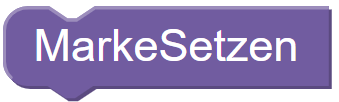
\includegraphics[height=25pt]{_Aufgaben/BlocksAndJava/img/markeSetzen.png}& \LoesungLine{karol.markeSetzen();}{1}\\

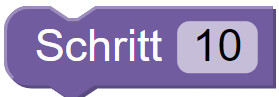
\includegraphics[height=25pt]{_Aufgaben/BlocksAndJava/img/step10.png}& \LoesungLine{karol.schritt(10);}{1}\\

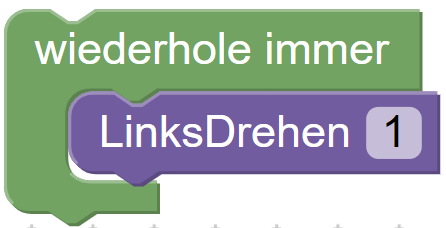
\includegraphics[width=\linewidth]{_Aufgaben/BlocksAndJava/img/whileTrue.png}&
\LoesungLine{while(true) \{ \newline \indent\hspace{1cm} karol.linksDrehen(1); \newline \} }{3}\\

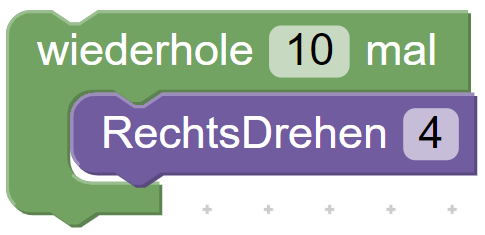
\includegraphics[width=\linewidth]{_Aufgaben/BlocksAndJava/img/for10.png}&\LoesungLine{for(int i=0; i < 10; i++) \{ \newline \indent\hspace{1cm} karol.rechtsDrehen(4); \newline \} }{3}

\end{tabularx}

\begin{tabularx}{\textwidth}{p{6cm}X}

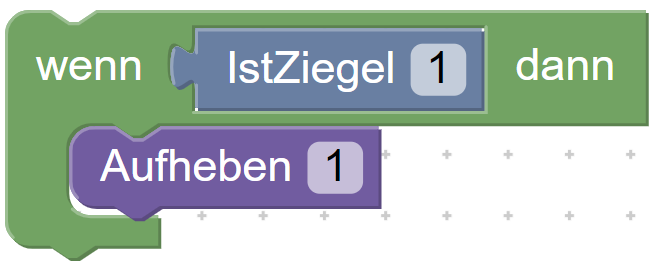
\includegraphics[width=\linewidth]{_Aufgaben/BlocksAndJava/img/if.png}& 
\LoesungLine{if(karol.istZiegel()) \{ \newline \indent\hspace{1cm} karol.aufheben(1); \newline \}}{3}\\\\

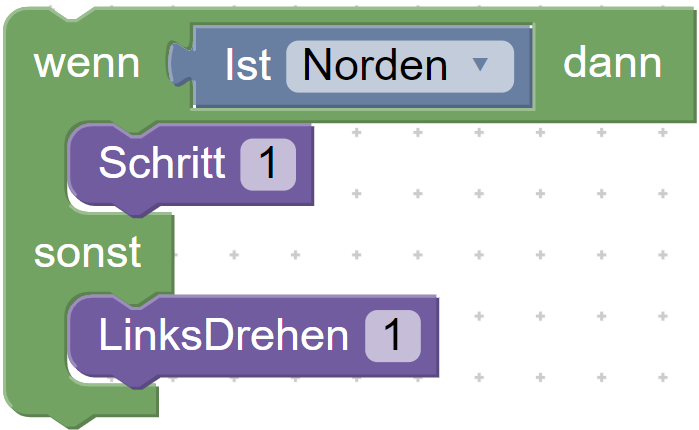
\includegraphics[width=\linewidth]{_Aufgaben/BlocksAndJava/img/ifelse.png}&
\LoesungLine{if(karol.istNordern()) \{ \newline \indent\hspace{1cm} karol.aufheben(1); \newline \} else \{ \newline \indent\hspace{1cm} karol.linksDrehen(1); \newline \}}{5}

\end{tabularx}

}

        \Hefteintrag{1.2}{Übersicht Befehlsarten}{
\label{sec:befehlsarten}

Es gibt viele verschiedene Befehlsarten. Die für uns wichtigsten sind:

\begin{tabularx}{\textwidth}{b{0.5cm}>{\centering\arraybackslash}b{3.5cm}>{\centering\arraybackslash}b{3.5cm}>{\centering\arraybackslash}X>{\centering\arraybackslash}X}
\emphColA{Art}
& \emphColA{Online-Karol} 
& \emphColA{Blockly} 
& \emphColA{Java} 
& \emphColA{Struktogramm} \\ 

%\rotatebox{90}{\Loesung{einf. Befehl\color{black}}{\lineheight}}

\LoesungLeer{\multicolumn{5}{l}{\color{blue} einf. Befehl\color{black}}\\}
%

&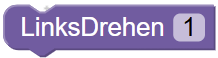
\includegraphics[width=\linewidth]{_Aufgaben//BlocklyJava_Skript//img/H02_karol_command.png}
&
\includegraphics[width=\linewidth]{_Aufgaben//BlocklyJava_Skript//img/H02_blockly_command.png}
&\LoesungKaro{karol.linksDrehen(1);\newline System.out.println("abc");}{4}
&\LoesungKaro{}{4}\\

\Loesung{\multicolumn{5}{l}{\color{blue} Verzweigung\color{black}}\\}

%\rotatebox{90}{\LoesungLine{Verzweigung}{1}}
&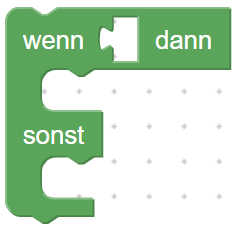
\includegraphics[width=\linewidth]{_Aufgaben//BlocklyJava_Skript//img/H02_karol_if-else.png}
&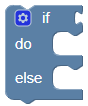
\includegraphics[width=2.5cm]{_Aufgaben//BlocklyJava_Skript//img/H02_blockly_if-else.png}
&\LoesungKaro{if(<Bedingung>) \{ \newline \indent\hspace{1cm} // wenn \newline \} else \{ \newline \indent\hspace{1cm} // sonst \newline \}}{7}
&\LoesungKaro{}{7}\\


\Loesung{\\\multicolumn{5}{l}{\color{blue} Schleife / bedingte Wiederholung\color{black}}\\}

%\rotatebox{90}{\LoesungLine{Schleife}{1}}
&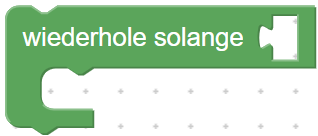
\includegraphics[width=\linewidth]{_Aufgaben//BlocklyJava_Skript//img/H02_karol_while.png}
&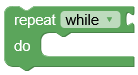
\includegraphics[width=\linewidth]{_Aufgaben//BlocklyJava_Skript//img/H02_blockly_while.png}
&\LoesungKaro{while(<Bedingung>) \{\newline...\newline\}}{5}
&\LoesungKaro{}{5}\\

\Loesung{\multicolumn{5}{l}{\color{blue} Zählschleife\color{black}}\\}

%\rotatebox{90}{\LoesungLine{Zählschleife}{1}}
&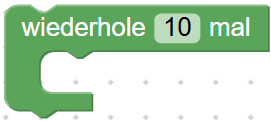
\includegraphics[width=\linewidth]{_Aufgaben//BlocklyJava_Skript//img/H02_karol_for.png}
&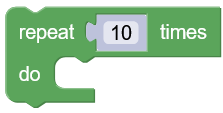
\includegraphics[width=\linewidth]{_Aufgaben//BlocklyJava_Skript//img/H02_blockly_for.png}
&\LoesungKaro{for(int i=0; i<10; i++) \{\newline...\newline\}}{7}
&\LoesungKaro{}{7}\\

\Loesung{\multicolumn{5}{l}{\color{blue} Methodendeklaration\color{black}}\\}

%\rotatebox{90}{\LoesungLine{M-Deklaration}{1}}
&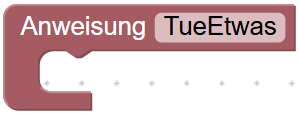
\includegraphics[width=\linewidth]{_Aufgaben//BlocklyJava_Skript//img/H02_karol_funcdef.png}
&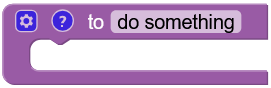
\includegraphics[width=\linewidth]{_Aufgaben//BlocklyJava_Skript//img/H02_blockly_funcdef.png}
&\LoesungKaro{public void doSomething() \{\newline...\newline\}}{5}
&\LoesungKaro{}{5}\\

\Loesung{\multicolumn{5}{l}{\color{blue} Methodenaufruf\color{black}}\\}

%\rotatebox{90}{\LoesungLine{M-Aufruf}{1}}
&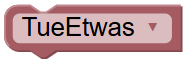
\includegraphics[width=\linewidth]{_Aufgaben//BlocklyJava_Skript//img/H02_karol_funccall.png}
&
\includegraphics[width=\linewidth]{_Aufgaben//BlocklyJava_Skript//img/H02_blockly_funccall.png}
&\LoesungKaro{doSomething();}{2}
&\LoesungKaro{}{2}\\

\Loesung{\\\multicolumn{5}{l}{\color{blue} Kommentar\color{black}}\\}

%\rotatebox{90}{\LoesungLine{Kommentar}{1}}
&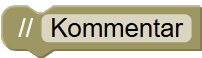
\includegraphics[width=\linewidth]{_Aufgaben//BlocklyJava_Skript//img/H02_karol_kommentar.png}
&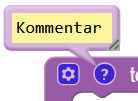
\includegraphics[width=0.8\linewidth]{_Aufgaben//BlocklyJava_Skript//img/H02_blockly_kommentar.png}
&\LoesungKaro{// Kommentar}{3}
&\LoesungKaro{}{3}\\


\Loesung{\\\multicolumn{5}{l}{\color{blue} Konstruktor\color{black}}\\}

%\rotatebox{90}{\LoesungLine{Konstruktor}{1}}
&%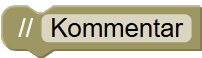
\includegraphics[width=\linewidth]{_Aufgaben//BlocklyJava_Skript//img/H02_karol_kommentar.png}
&
\includegraphics[width=1.1\linewidth]{_Aufgaben//BlocklyJava_Skript//img/H02_blockly_ctrdef.png}
&\LoesungKaro{public MeineKlasse() \{\newline...\newline\}}{4}
&\LoesungKaro{}{4}\\


\Loesung{\multicolumn{5}{l}{\color{blue} Objekt erstellen\color{black}}\\}

%\rotatebox{90}{\LoesungLine{Objekt erstellen}{1}}
%&%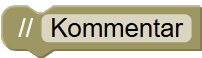
\includegraphics[width=\linewidth]{_Aufgaben//BlocklyJava_Skript//img/H02_karol_kommentar.png}
&
&
\includegraphics[width=1.1\linewidth]{_Aufgaben//BlocklyJava_Skript//img/H02_blockly_ctrcall.png}
&\LoesungKaro{new MeineKlasse();}{2}
&\LoesungKaro{}{2}\\

\end{tabularx}

}
    }

    \mysession{Stunde 3+4}{
        \Aufgabe{Semikolon und geschweifte Klammern}

Wann macht man in Java ein Semikolon und wann setzt man geschweifte Klammern ein?

\begin{enumerate}
    \item Überlege zuerst allein (2 Minuten)
    \item Besprecht eure Überlegungen zu zweit und probiert sie in Online-Karol zur bestätigen (4 Minuten)
\end{enumerate}


        \Hefteintrag{1.7}{Strukturierung von Programmcode - Syntax}{

In Java wird Programmcode vor allem mit \emphColA{\LoesungLuecke{Semikolons und geschweiften Klammern}{10cm}} strukturiert:

\doppelseite{0.55}{0.4}{t}{%
\begin{itemize}
    \item \LoesungLuecke{Semikolons}{5cm}~markieren das Ende eines \emphColA{einfachen Befehls oder Methodenaufrufs} (normalerweise am Ende der Zeile).
    \item \LoesungLuecke{Geschweifte Klammern}{7cm}~markieren \emphColA{Code-Abschnitte}, die wiederholt (Schleifen) oder bedingt (Bedingung) ausgeführt werden. Außerdem markieren sie den Methodenrumpf und Anfang und Ende einer Klasse. Je nachdem, was durch die Klammern markiert wird, spricht man synonym zu \LoesungLuecke{innerhalb}{5cm}~der Klammern auch von \LoesungLuecke{innerhalb}{5cm}~der Klasse, Methode, Schleife, etc.
\end{itemize}
}{%
\centering

\includegraphics[width=\linewidth]{_Aufgaben/BlocklyJava_Skript/img/H03_semicolonMeme.png}
\scriptsize www.reddit.com/r/ProgrammerHumor/comments/o0anud/semicolon}
}


        \Hefteintrag{2}{Strukturierung von Programmcode - Semantik: Methoden}{%

Beim Programmieren können eigene Anweisungen/ Befehle/ Methoden/ Funktionen \textbf{deklariert} werden. Bei der \textbf{Deklaration beschreibt} zunächst mit dem \LoesungLuecke{Methodenkopf}{6cm}, welche Eigenschaften die Methode hat und anschließend im \LoesungLuecke{Methodenrumpf}{6cm}, wie genau sie sich verhalten soll. Eine deklarierte Methode kann anschließend beliebig oft verwendet (=\emphColA{aufgerufen}) werden.

Hierdurch kann man sehr lange Programme in übersichtlichere Einzelteile zerlegen, sodass \LoesungLuecke{doppelter Code}{8cm}~reduziert wird, der Code durch aussagekräftige \LoesungLuecke{Methodennamen}{6cm}~besser verstanden werden kann und Fehler schneller gefunden werden.

In Java darf außerdem kein auszuführender Programmcode außerhalb von Methoden sein.

Die Deklaration besteht aus \emphColB{Methodenkopf} und \emphColC{Methodenrumpf} (von geschweiften Klammern umschlossen):

{\ttfamily
\emphColB{void tueEtwas()} \emphColC{\{}

~~~~\emphColC{karol.schritt(2);}
    
\emphColC{\}}
}

Der \emphColA{Aufruf} funktioniert wie ein einfacher Befehl: 

\emphColA{\texttt{tueEtwas();}}

}

        \Aufgabe{Übersetzungstraining: Methoden}{

Übersetze die folgenden Code-Schnippsel (\emph{code snippets}) in Java-Code ohne den Computer zu verwenden.

\begin{center}
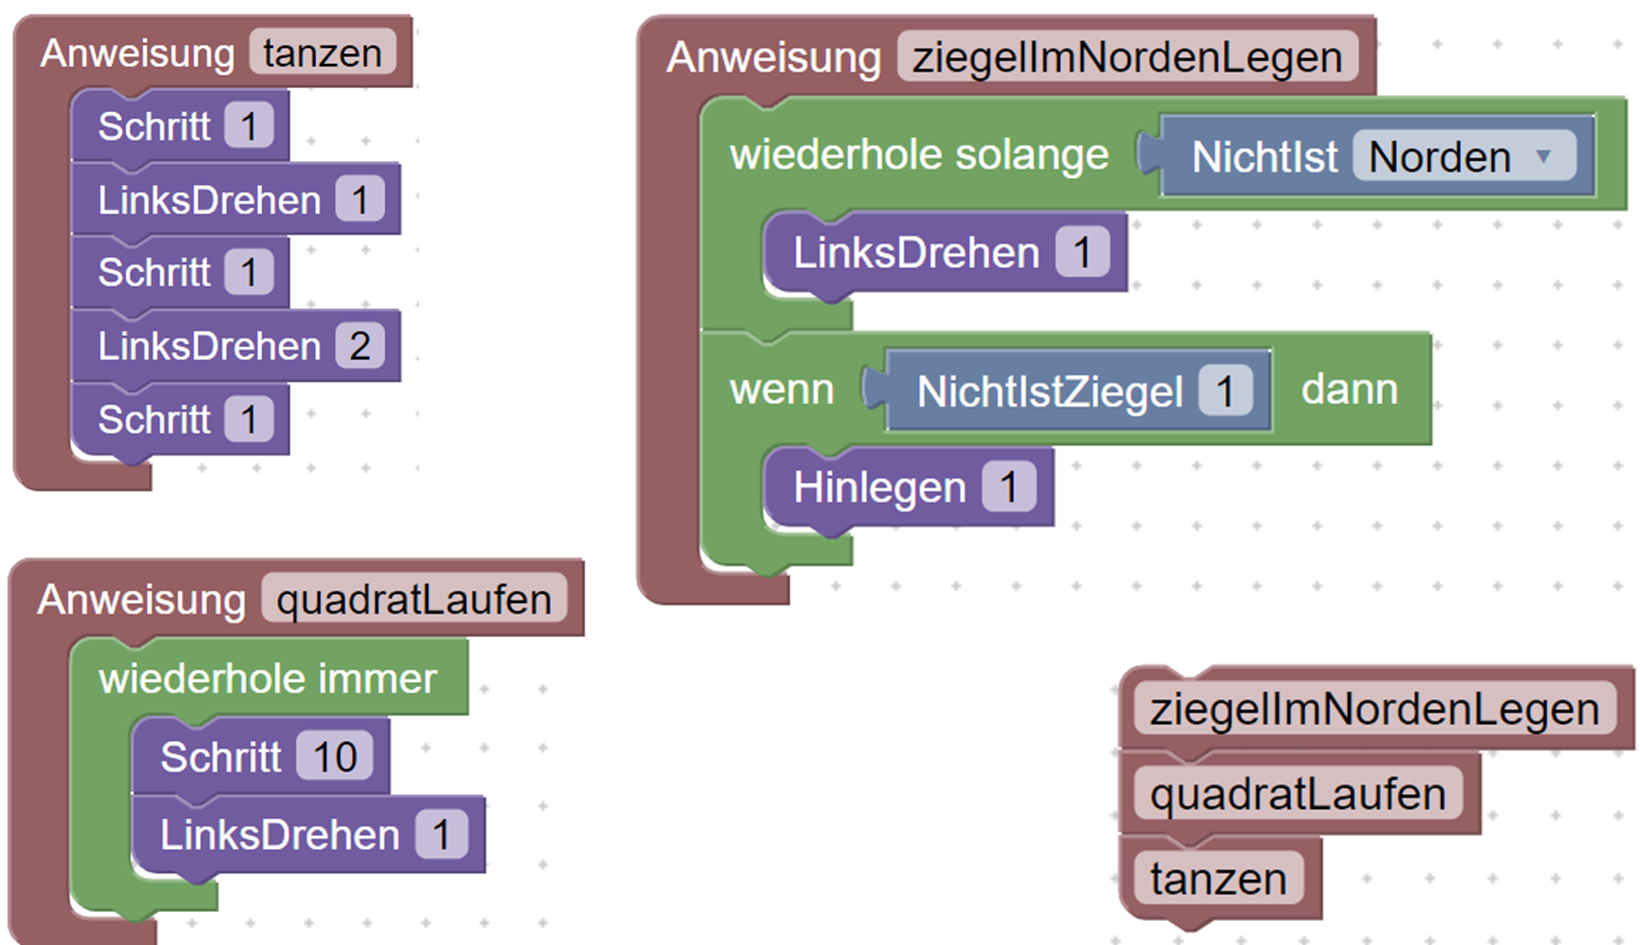
\includegraphics[width=0.75\textwidth]{_Aufgaben/BlocklyJava_Skript/img/A03_transMethods.png}
\end{center}


\LoesungKaro{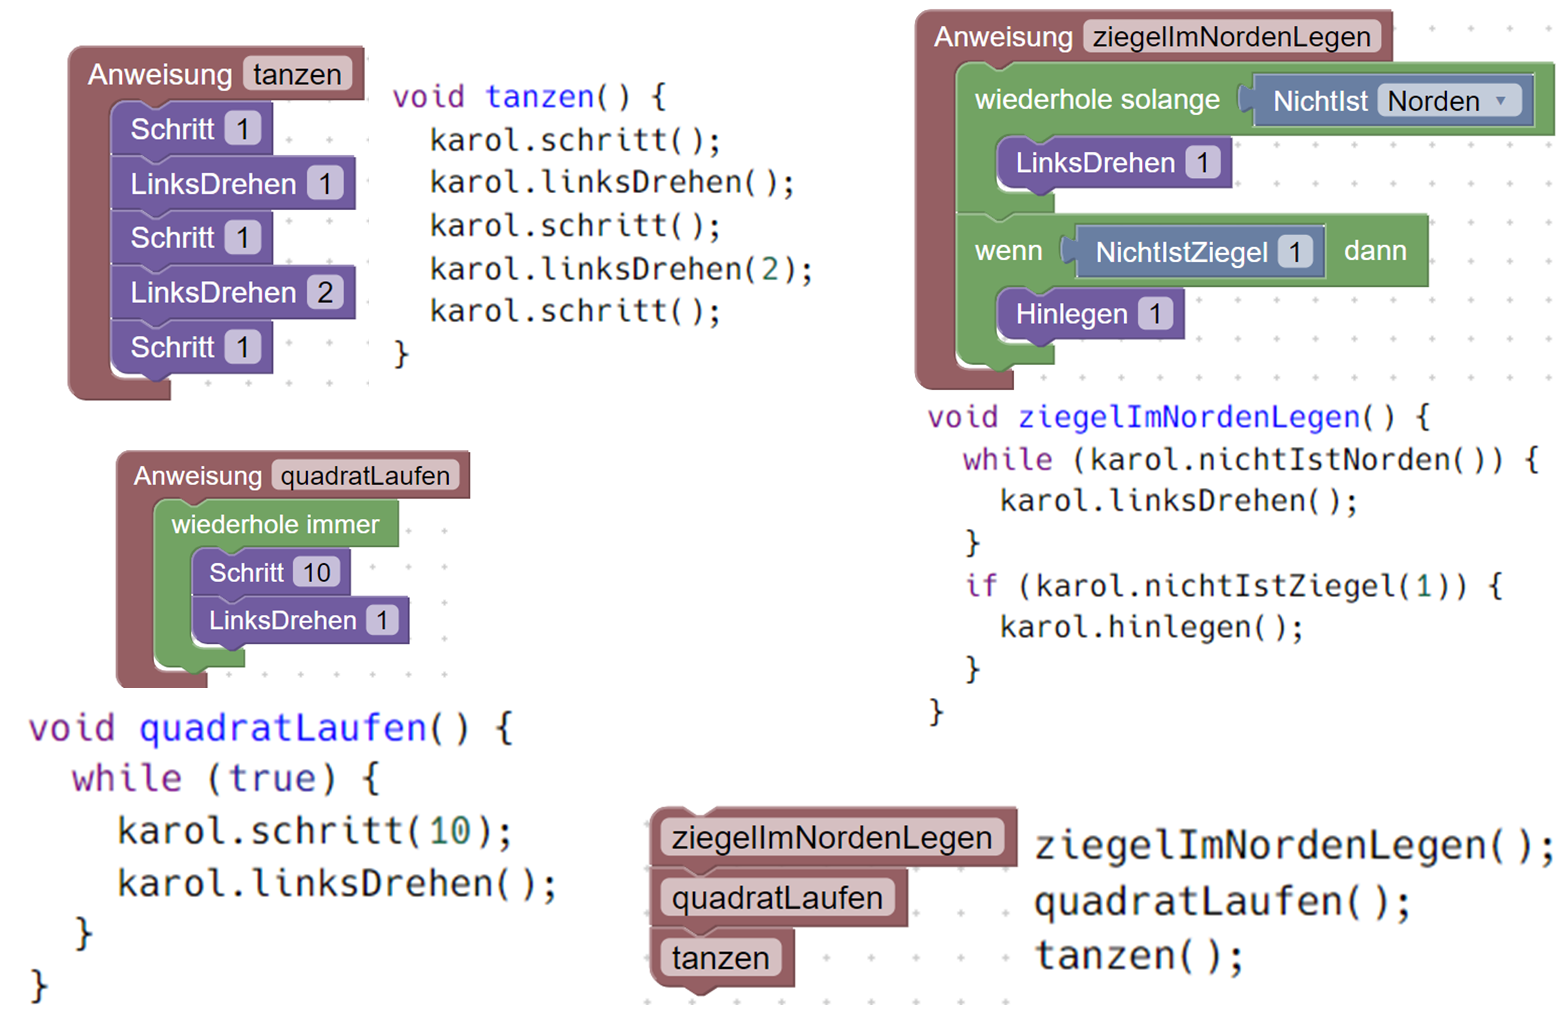
\includegraphics[width=\textwidth]{_Aufgaben/BlocklyJava_Skript/img/A03_transMethods_sol.png}}{32}
}

        \Aufgabe{Karol mit Java und Struktogramme}

\doppelseite{0.55}{0.3}{t}{%
\begin{itemize}
    \item Bearbeite die Robot Karol (\url{karol.arrrg.de}) Level erneut. Schreibe den Programmcode dieses Mal direkt in Java!\\
    Zur Erinnerung: Deinen Code schreibst du an der gelb markierten Stelle in der main-Methode.
    \item Zeige nach den Schritten jeweils das Struktogramm an und notiere auf einem \emphColB{Schmierzettel}, wie du die letzte Spalte in Hefteintrag \ref{sec:befehlsarten} befüllen würdest.
    \item Was passiert, wenn du dein Programm aus eigenen Methoden aufbaust? Wieso ist das so?
\end{itemize}

}{%
 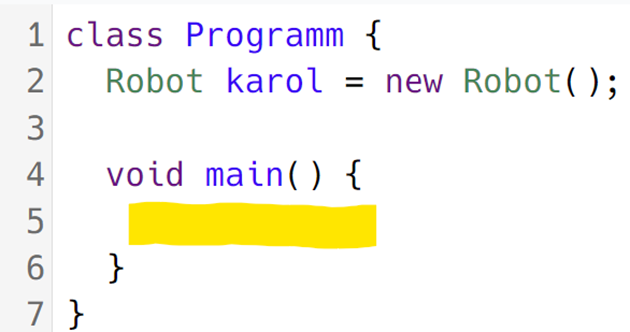
\includegraphics[width=\linewidth]{_Aufgaben/BlocklyJava_Skript/img/A04_karol_mainMarkiert.png}
 
 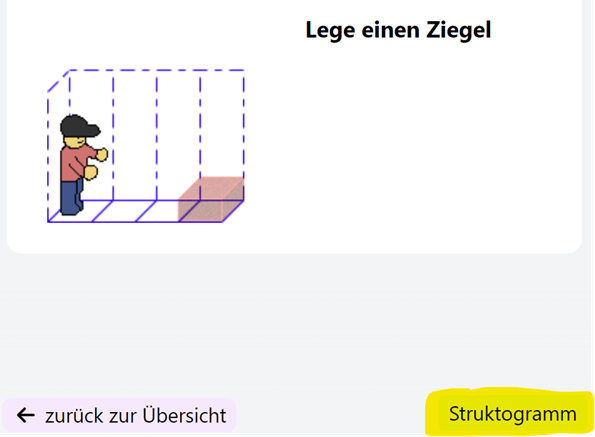
\includegraphics[width=\linewidth]{_Aufgaben/BlocklyJava_Skript/img/A04_karol_struktoMarkiert.png}
}


    }
    \mysession{Stunde 5}{

        \Hefteintrag{2}{Programmablauf grafisch darstellen: Struktogramme}{%
Struktorgramme (auch: \LoesungLuecke{Nassi-Shneiderman-Diagramme}{12cm}) stellen \emphColA{Algorithmen (=Ablauf eines Programms)} grafisch dar. Ein Struktogramm bezieht sich immer auf genau eine Methode und stellt aufgerufene Methoden als ein Element dar.

In \textbf{Hefteintrag \ref{sec:befehlsarten}} sind die Struktogramm-Bausteine für verschiedene Befehlsarten dargestellt, die beliebig miteinander kombiniert werden können. 

Zusätzlich gibt es folgenden Baustein, der eine leere Stelle (z.B. leerer else-Block) darstellt:

\vspace{4cm}


}

        \Aufgabe{Struktogramm-Training}{

Zeichne zu den folgenden Code Snippets jeweils ein Struktogramm:

\begin{center}
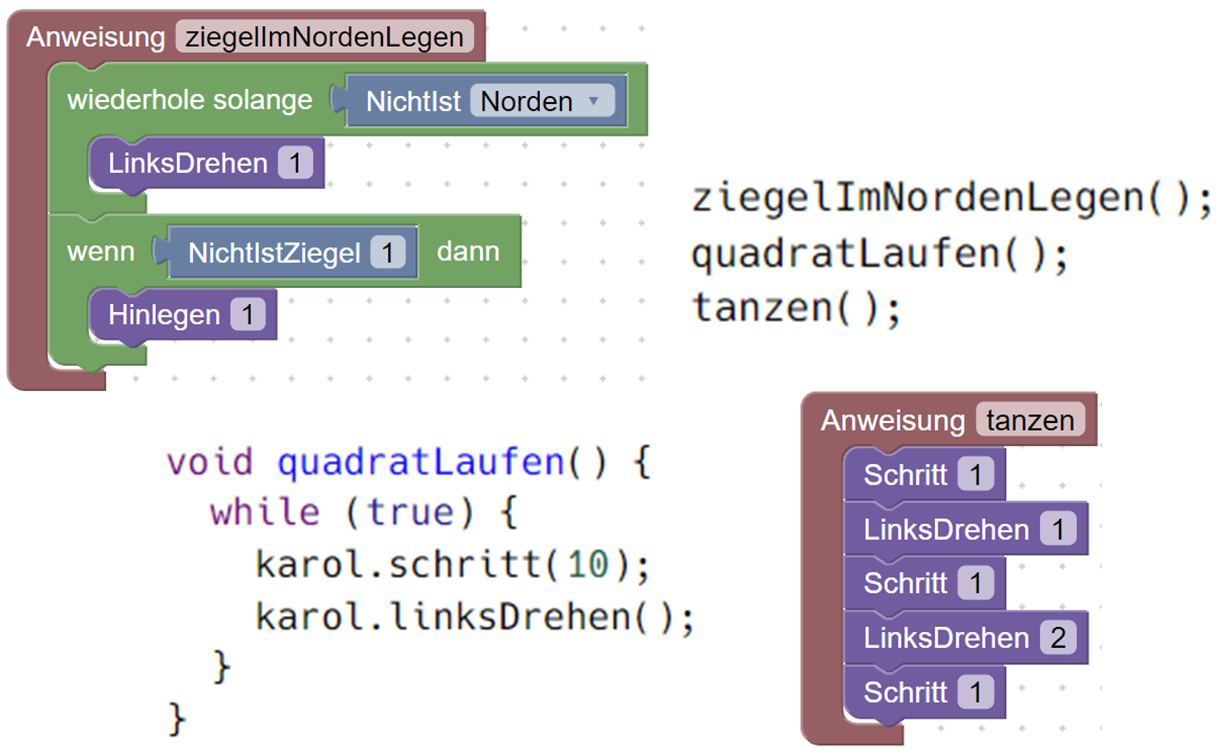
\includegraphics[width=0.75\textwidth]{_Aufgaben/BlocklyJava_Skript/img/A05_transMethods_strukto.png}
\end{center}


\LoesungKaro{}{29}
}
    }

    \mysession{Stunde 6+7}{

        \section{Taschenrechner}

\flushleft

\begin{minipage}{0.49\textwidth}
Implementiere das Klassendiagramm rechts mit Hilfe von Blockly. Probiere deine Methode aus (siehe Anleitung auf der Vorderseite). Fülle die Lücken im Java-Code unten aus, wenn deine Methoden funktionieren.
\end{minipage}
\hfill
\begin{minipage}{0.49\textwidth}
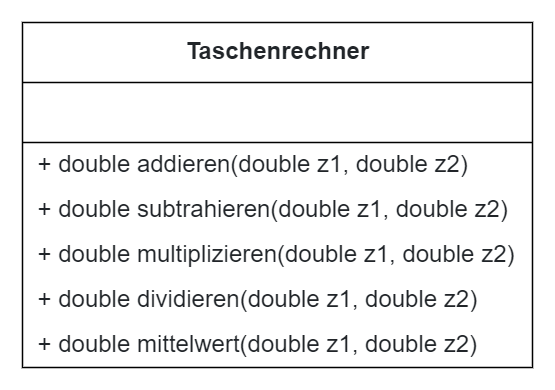
\includegraphics[width=\linewidth]{_Aufgaben/BlocksAndJava/img/Taschenrechner.png}
\end{minipage}

\LARGE


\begin{lstlisting}[escapechar=\&]

public class Taschenrechner
{    
    public & \LoesungLuecke{double addieren(double z1, double z2) \{ }{12cm} &
        
            & \LoesungLuecke{return z1 + z2;}{12cm} &
    }
    public &\LoesungLuecke{double subtrahieren(double z1, double z2) \{ }{12cm}&
        
            & \LoesungLuecke{return z1 - z2;}{12cm} &
    }
    public &\LoesungLuecke{double multiplizieren(double z1, double z2) \{ }{12cm}&
        
            & \LoesungLuecke{return z1 * z2;}{12cm} &
    }
    public & \LoesungLuecke{double dividieren(double z1, double z2) \{ }{12cm}&
        
            & \LoesungLuecke{return z1 + z2;}{12cm} &
    }
    public & \LoesungLuecke{double mittelwert(double z1, double z2) \{ }{12cm} &
        
            & \LoesungLuecke{return (z1 + z2) / 2;}{12cm} &
    }
}
\end{lstlisting}
        
        \Hefteintrag{2}{Methodenköpfe}{%

Im \LoesungLuecke{Methodenkopf}{8cm} können neben dem Namen noch weitere Informationen nach folgendem Schema gespeichert werden: 

\emphColB{Zugriffsmodifizierer} \emphColA{Rückgabetyp} \emphColC{name}(\emphColA{Datentyp} \emphColC{parametername}) \{ //... \}


\emphColB{public} \emphColA{void} \emphColC{schritteLaufen}(\emphColA{int} \emphColC{anzahl}, ...) \{ //... \}

\vspace{0.5cm}

Methodenname und Parametername können weitgehend frei gewählt werden (Groß- und Kleinschreibung beachten!). Folgendes ist \textbf{nicht} erlaubt:
\LoesungLine{Leerzeichen im Namen, Zahlen am Anfang des Namens, Rechenzeichen im Namen, Schlüsselwörter als Name}{3}

\vspace{0.5cm}

Die verwendeten \LoesungLuecke{Schlüsselwörter}{8cm} haben folgende Bedeutungen:

\emphColB{Zugriffsmodifizierer: public} - Methode kann ‚überall‘ verwendet werden. (im Gegensatz dazu \emph{private}: nur in der gleichen Klasse)

\emphColA{Datentyp} - Art der Daten (z.B. Ganzzahlen: \LoesungLuecke{int}{2cm}, Kommazahlen: \LoesungLuecke{double}{3cm}, Text: \LoesungLuecke{String}{3cm}, Wahrheitswert: \LoesungLuecke{boolean}{4cm})

\emphColA{Rückgabetyp} - Datentyp des Rückgabewerts (=\LoesungLuecke{return-value}{7cm}). Kann z.B. Ergebnis einer Berechnung sein. 

\emph{Besonderer Rückgabetyp} - \emph{void} bedeutet, die Methode hat keinen Rückgabewert. Außer bei void wird immer eine return-Anweisung benötigt.

\textbf{Parameter} - Speichert bei jedem Aufruf einen neuen Wert, der im Methodenrumpf über den Namen verwendet werden kann.


}

        \Hefteintrag{2}{Methoden im Klassendiagramm}{%

\doppelseite{0.42}{0.52}{t}{%
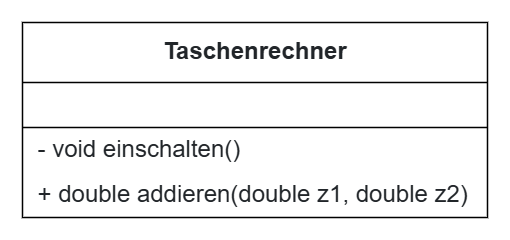
\includegraphics[width=\linewidth]{_Aufgaben//BlocklyJava_Skript//img/H07_KD.png}
}{%
    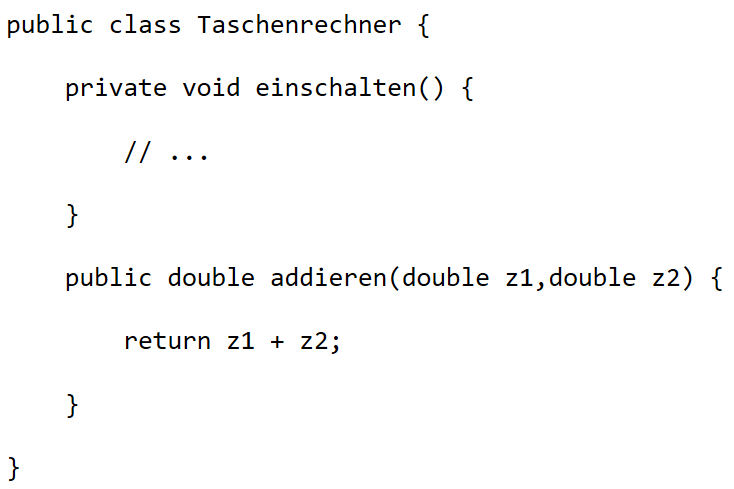
\includegraphics[width=\linewidth]{_Aufgaben//BlocklyJava_Skript//img/H07_Code.png}
}
}


        \Aufgabe{Attribute im Klassendiagramm}{

Findet heraus, wie Attrbiute im Klassendiagramm dargestellt werden. Achtet auf \emphColB{Zugriffsmodifizierer, Datentyp und Name}. Macht eine Skizze auf einem Schmierblatt.

}

        \Hefteintrag{2}{Attribute im Klassendiagramm}{%
Attribute werden im Klassendiagramm folgendermaßen dargestellt:

\centering
\vspace{1cm}
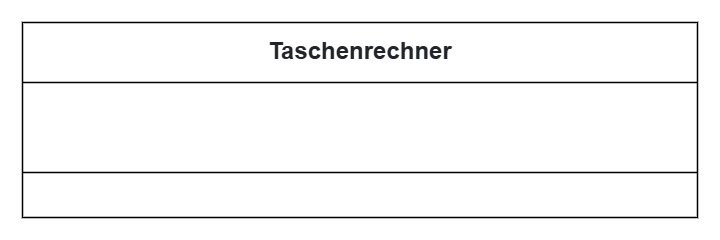
\includegraphics[width=0.7\textwidth]{_Aufgaben/BlocklyJava_Skript/img/H08_KD.png}


\vspace{1cm}

}

        
\begin{minipage}[t]{\textwidth}
\Aufgabe{Struktogramme und Klassendiagramme}

\textbf{Setze folgende Diagramme in BlueJ-Blockly um und notiere den Programmcode auf der nächsten Seite}

\vspace{0.5cm}

\doppelseite{0.45}{0.5}{t}{%
\textbf{Klassendiagramm:}

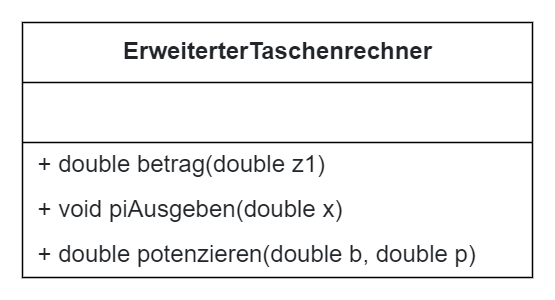
\includegraphics[width=\linewidth]{_Aufgaben/BlocksAndJava/img/klasse.png} 
}{%

\textbf{Struktogramm für piAusgeben(double x):}

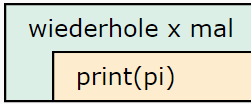
\includegraphics[width=0.6\linewidth]{_Aufgaben/BlocksAndJava/img/strukt_10pi.png}
}

\vspace{1cm}

\textbf{Zeichne hier die Struktogramme für die restlichen Methoden:}

\LoesungKaro{\\
\Large
+ double betrag(double z1) \\
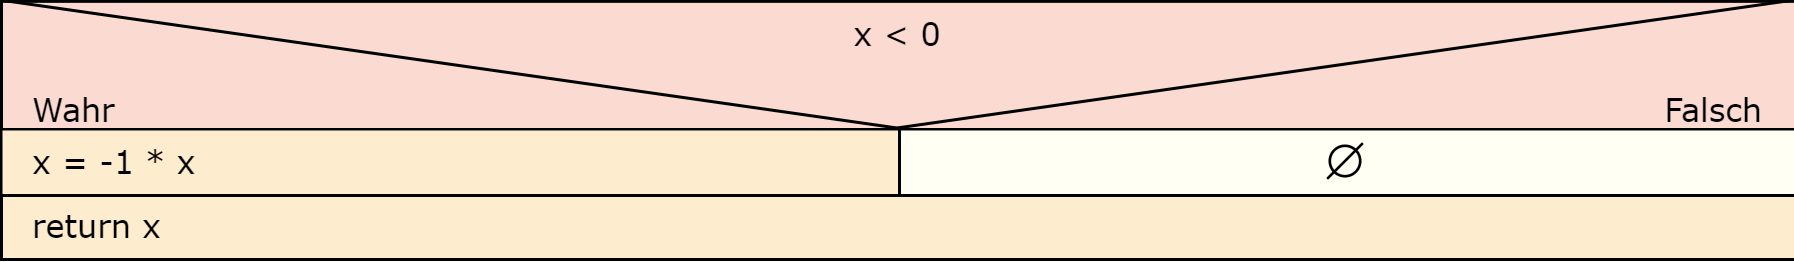
\includegraphics[width=\textwidth]{_Aufgaben/BlocksAndJava/img/strukt_betrag.png} \\\\
+ double potenzieren(double b, double p) \\
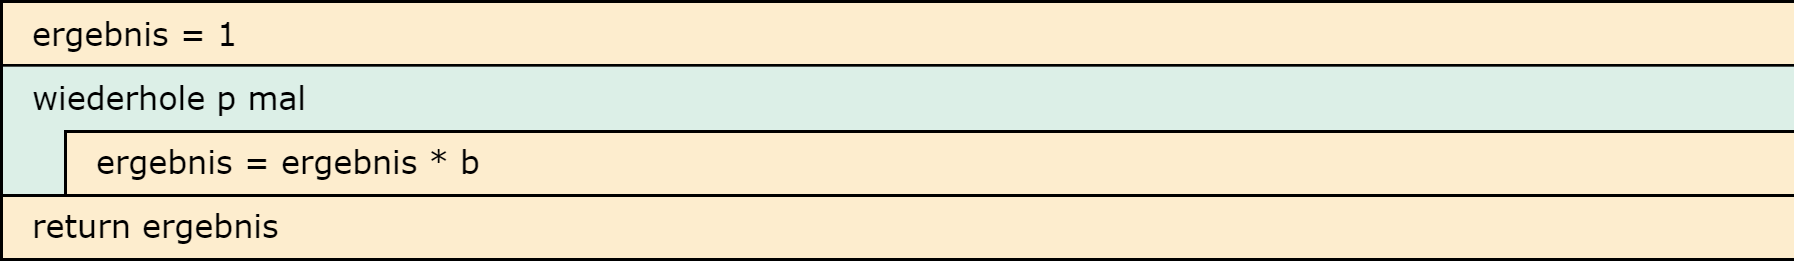
\includegraphics[width=\textwidth]{_Aufgaben/BlocksAndJava/img/strukt_protenz.png}}{25}

    
\end{minipage}


\begin{minipage}[t]{\textwidth}
\Large
\begin{lstlisting}[escapechar=\&]
public class ErweiterterTaschenrechner
{    
    public & \LoesungLuecke{double betrag(double z1) \{ }{15cm} &
    
        & \LoesungLuecke{if(z1 < 0) \{ }{15cm} &
        
            & \LoesungLuecke{z1 = -1 * z1;}{15cm} &
            
        & \LoesungLuecke{\}}{15cm} &   
        
        & \LoesungLuecke{return z1;}{15cm} &   
    }
    public & \LoesungLuecke{void piAusgeben(double x) \{ }{15cm} &
    
        & \LoesungLuecke{for(int i=0; i < x; i++) \{ }{15cm} &
        
            & \LoesungLuecke{System.out.println(Math.PI);}{15cm} &
            
        & \LoesungLuecke{\}}{15cm} &
    }
    public & \LoesungLuecke{double potenzieren(double b, double p) \{ }{15cm} &

        & \LoesungLuecke{double ergebnis = 1.0;}{15cm} &
    
        & \LoesungLuecke{for(int i=0; i < p; i++) \{ }{15cm} &
        
            & \LoesungLuecke{ergebnis = ergebnis * b;}{15cm} &
            
        & \LoesungLuecke{\}}{15cm} &
            
        & \LoesungLuecke{return ergebnis;}{15cm} &
    }
}
\end{lstlisting}

\end{minipage}
        
    }
}